\chapter{Project Development}\label{ch:project-development}

This chapter provides an in-depth look into the development of Chronocademy, outlining the key aspects that contributed to its creation.
The following sections will cover essential areas of the project, including product development, user experience, developer experience, the technologies used, and the code architecture.

Each of these areas played a critical role in shaping Chronocademy into a functional and user-friendly platform.
From defining the product's core features and refining its usability to selecting the right tools and structuring the codebase, this chapter highlights the processes and decisions that guided the project from concept to development.

By exploring these topics, the reader will gain a comprehensive understanding of how the team approached the challenges of building Chronocademy and the methods they used to ensure a robust, scalable, and well-designed platform.

\section{Product Development}\label{sec:productdevelopment}
The development of Chronocademy began by defining, refining, and prioritizing its core aspects and features.
This section outlines the step-by-step process undertaken to shape the product, ensuring it was both viable and aligned with the needs of its users.

\subsection{Defining the Idea through the Business Model Canvas}\label{subsec:business-model-canvas}
The first step in the product development journey was to define the core idea behind Chronocademy.
To structure and validate this concept, the team utilized the Business Model Canvas framework.

\begin{quote}
    ``The Business Model Canvas is a strategic management and entrepreneurial tool.
    It allows you to describe, design, challenge, invent, and pivot your business model.
    This method from the bestselling management book Business Model Generation is applied in leading organizations and start-ups worldwide.''
\end{quote}\cite{business-canvas-model}

This tool helped identify the key components of the platform, including the value proposition, target customer segments, revenue streams, cost structure, among others.
By analyzing these elements, the team was able to understand how Chronocademy would create, deliver, and capture value in a competitive landscape.
The structured approach of the Business Model Canvas ensured that the idea was not only innovative but also practical and sustainable.

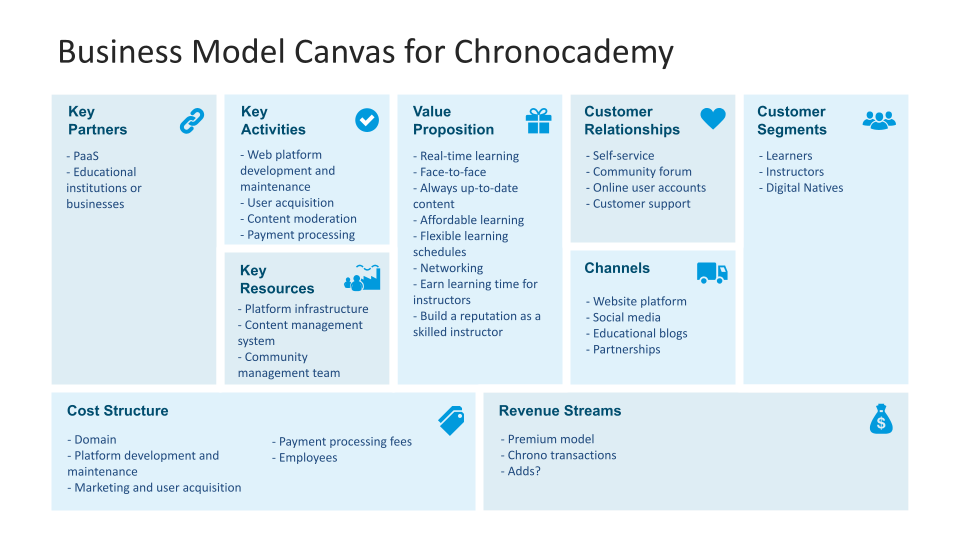
\includegraphics[width=14cm]{business-canvas-model}

\underline{Key resources:}
\begin{itemize}
\item Online platform infrastructure: Website development and maintenance for user accounts, course listings, scheduling, and video conferencing.
\item Content management system (CMS): A system to allow instructors to upload course descriptions and materials.
\item Community management team: Answer to user requests, ensure a positive learning environment and moderate.
\end{itemize}

\underline{Key activities:}
\begin{itemize}
\item Web platform development and maintenance: Develop and continuously update and improve the website for optimal user experience.
\item User acquisition: Marketing strategies to attract users.
\item Content moderation: Moderate courses to ensure quality.
\item Payment processing: Implement a secure system for handling transactions.
\end{itemize}

\underline{Key partnerships:}
\begin{itemize}
\item Video conferencing platform: Integrate a reliable video conferencing service for online lessons.
\item Educational institutions or businesses.
\item Payment processing companies: Integrate a secure payment processor.
\end{itemize}

\underline{Value propositions:}
\begin{itemize}
\item Real-time learning face-to-face: Access to a wide range of skills and knowledge from instructors in real-time face-to-face.
\item Always up-to-date content.
\item Affordable learning: Main payment goes through a time-based exchange system.
\item Flexible learning schedules: Using calendars and through online video conferencing.
\item Networking: Opportunity to connect with a community of learners and instructors.
\item Earn learning time for instructors: Then can be used to acquire new skills and knowledge themselves.
\item Build a reputation as a skilled instructor: Thanks to students feedback and ratings.
\end{itemize}

\underline{Customer relationships:}
\begin{itemize}
\item Self-service: Learners and instructors can work autonomous.
\item Community forum: Create a forum for learners and instructors to interact, ask questions, and share experiences.
\item Online user accounts: Users will create accounts to manage their learning time, browse courses, schedule lessons, and provide feedback.
\item Customer support: Offer email or chat support for users encountering technical difficulties, needing assistance or providing feedback.
\end{itemize}

\underline{Customer segment:}
\begin{itemize}
\item Learners: Persons trying to acquire new knowledge through real-time instruction.
\item Instructors: Persons with expertise willing to share their knowledge and earn learning time.
\item Digital natives.
\end{itemize}

\underline{Channels:}
\begin{itemize}
\item Website: Primary channel for user registration, course browsing, lesson scheduling, and video conferencing.
Centralised platform.
\item Social media: Used for marketing, promotion, and building a community around Chronocademy.
\item Educational blogs or partnerships: Collaborate with educational blogs or platforms to promote Chronocademy and reach potential learners.
\end{itemize}

\underline{Cost structure:}
\begin{itemize}
\item Domain: Pay and maintain the internet domain over time.
\item Platform development and maintenance: Costs associated with website development, hosting, and ongoing maintenance.
\item Marketing and user acquisition: Costs for online advertising and social media marketing.
\item Content moderation: Costs associated with managing the course submission process and ensuring lessons quality.
\item Payment processing fees: Fees charged by payment processors for handling transactions.
\item Community management team: Costs associated with management of the online community.
\end{itemize}

\underline{Revenue streams:}
\begin{itemize}
\item Premium model: It offers free Chrono, access to exclusive lessons scripts and a better advertisement for teachers.
\item Chrono transactions: Charge for transactions fees either for buying or selling Chronos.
\item Ads: Include ads (not very intrusive).
\end{itemize}

After completing the Business Model Canvas, the team had a clear understanding of the platform's value proposition, target audience, revenue streams, and cost structure.
This work laid the groundwork for the subsequent stages of product development.

\subsection{Establishing the Brand: Colors, Logo, and Slogans}\label{subsec:colors-logo-slogans}
With the foundation of the business model in place, the second step was establishing a unique and memorable brand identity for Chronocademy.
The team selected a color palette that reflected the platform’s values of knowledge, reliability and accessibility.
The logo was designed to be simple yet distinctive, incorporating elements that represent time spent on learning and growth.
As well as the name, Chronocademy, which combines the words ``chronos'' (latin for time) and ``academy'' to emphasize the platform's focus on real-time learning.
Slogans were thought to be a good match with the platform, such as ``Learn.
Teach.
Grow.'' These branding efforts were crucial for creating a meaningful identity with the target audience and set Chronocademy apart in the market.

\subsubsection{Color Palette}\label{subsubsec:color-palette}
The color palette for Chronocademy was chosen following the colors theory, which is

\begin{quote}
``a set of practices for picking colours together for harmonious designs and contextual combinations''
\end{quote}\cite{colorTheory}.

The first step was to decide which tone of colors would be used, and the team decided to use some warm colors to give a sense of energy and modern product instead of pastel colors, which are know for their calming and trustworthy interpretation.

Once the color analysis was defined, the team started to work on the style tiles to actually pick the exact colors for the brand.
Style tiles are a design tool defined as:

\begin{quote}
``a design deliverable consisting of fonts, colors and interface elements that communicate the essence of a visual brand for the web
[\ldots]
They help form a common visual language between the designers and the stakeholders and provide a catalyst for discussions around the preferences and goals of the client.
[\ldots]
Style tiles establish a direct connection with actual interface elements without defining layout.''
\end{quote}\cite{styleTiles}

The first step to build the style tile board was to define the concept: \textit{``knowledgeable, reliable, and accessible''}.
Then, we searched for images and illustrations that would represent those words and extract the colors out of them.
By doing this a couple of times, we ended up with two different style tiles that were combined to create the final one, by using the fonts of tile number 1 and colors of tile number 2.\newline

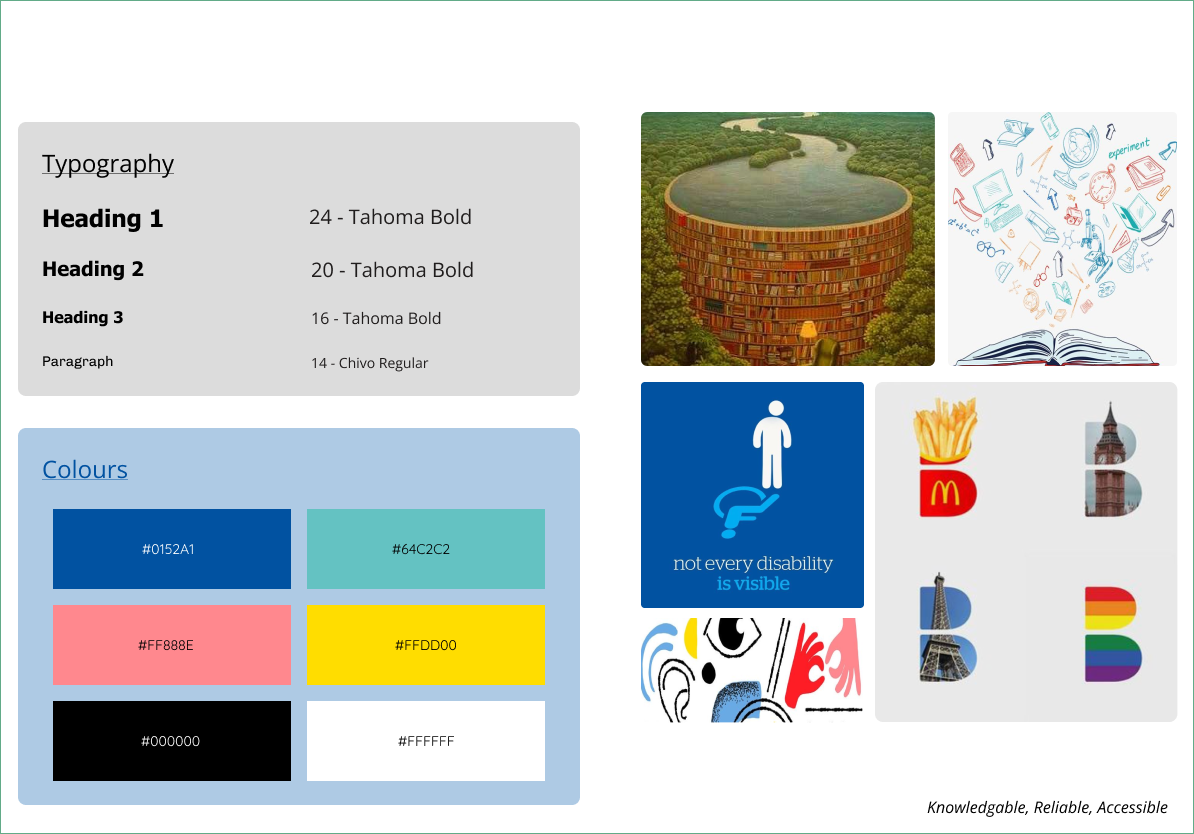
\includegraphics[width=14cm]{style-tile-1}\newline
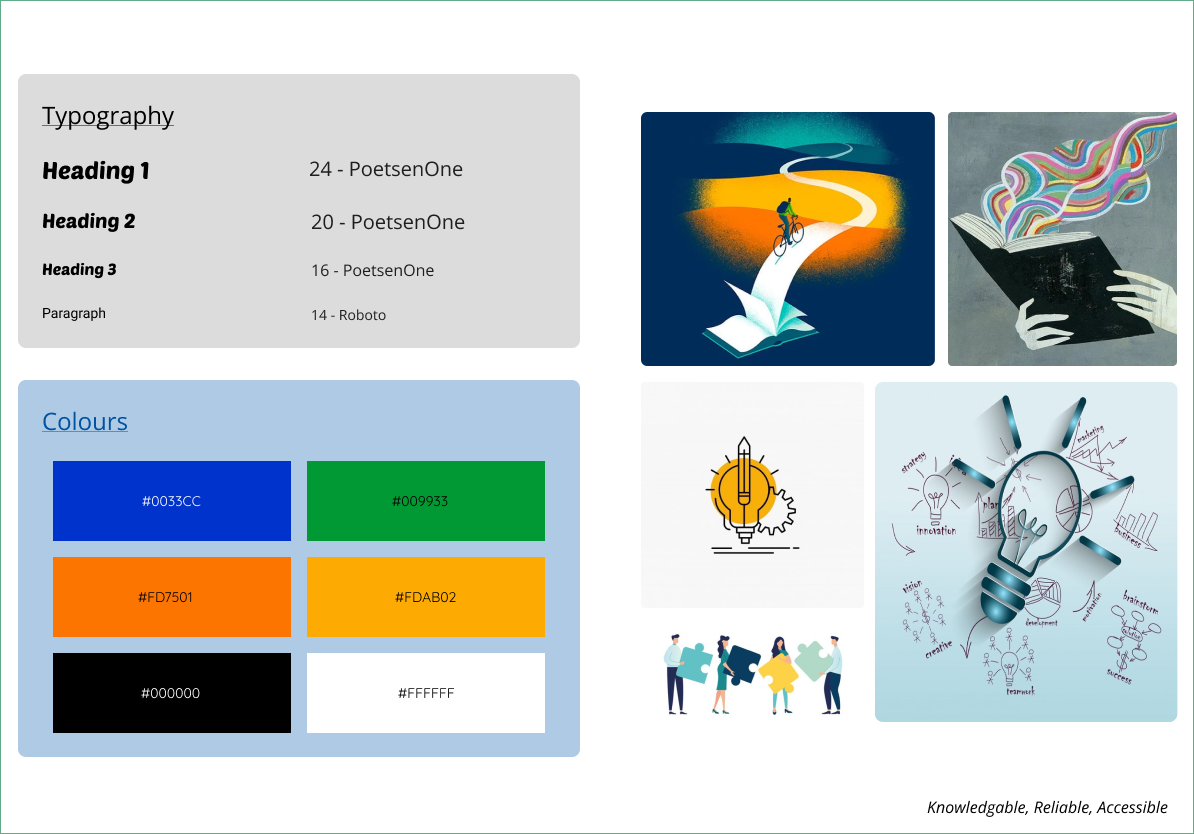
\includegraphics[width=14cm]{style-tile-2}\newline

This tool was helpful to come up with the final color palette and fonts that would be used in the platform.
The final style tile board is shown below.
All three versions were focused on the same concept of \textit{``knowledgeable, reliable, and accessible''}.\newline

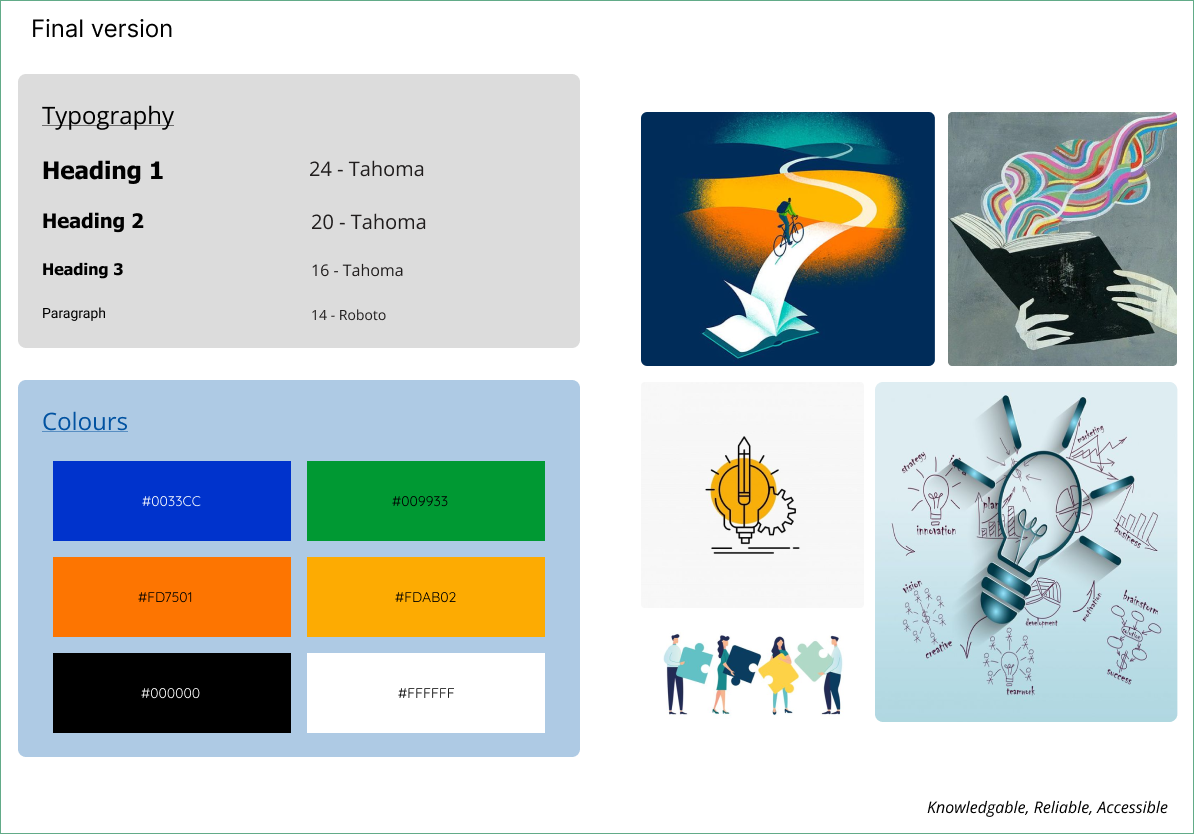
\includegraphics[width=14cm]{style-tile-final}\newline

\subsection{Defining the Target Audience}\label{subsec:target-audience}

The third step in the product development process was identifying the target audience for Chronocademy, including their characteristics, preferences, and strategies for attracting and retaining them.
The target audience consists of the following groups:

\begin{itemize}
    \item \underline{Learners Only}: These users are interested in acquiring new skills but have no interest or time to teach.
    They prefer structured, face-to-face learning with specific goals in mind and have the financial means to purchase Chrono tokens.
    Strategies to attract them include highlighting the option to buy Chronos and showcasing the platform’s variety of classes and user-friendly features.
    Retention methods include offering high-quality courses, loyalty programs, progress tracking, and a community space for sharing experiences.
    \item \underline{Teachers Only}: These users focus on sharing knowledge and earning Chrono but are not interested in learning.
    They are often experienced educators motivated by the flexibility and financial incentives of the platform.
    To attract them, the emphasis should be on earning Chronos, success stories, and ease of use.
    Retention strategies include resources for teaching improvement, certifications, and a supportive community.
    \item \underline{Teachers and Learners}: This group enjoys both learning and teaching, motivated by personal development and the opportunity to share knowledge.
    Attracting them requires emphasizing the dual benefits of earning and spending Chronos.
    Retention strategies focus on providing balanced incentives, such as personalized recommendations and recognition for active participation in both roles.
    \item \underline{Casual Learners}: These users are hobbyists learning for personal enjoyment without a structured schedule.
    They value flexibility and variety.
    Social media advertising and testimonials can help attract this group, while retention depends on expanding skill offerings and supporting flexible learning.
    \item \underline{Professional Learners}: These users aim to advance their careers or professional skills.
    They are willing to invest time and money for high-quality learning.
    Highlighting career benefits and using professional networks like LinkedIn can attract them, while retention relies on offering specialized teachers and networking opportunities.
    \item \underline{Casual Teachers}: These individuals teach for enjoyment or extra income without a professional teaching background.
    They are motivated by their passion for sharing knowledge.
    Strategies to attract them include emphasizing the rewarding aspects of teaching and using social media to engage hobbyists.
    Retention strategies mirror those for professional teachers but include additional support for casual teaching improvements.
    \item \underline{Professional Teachers}: Users with formal training or significant teaching experience who teach as a primary or secondary profession.
    Attracting this group involves promoting the platform’s quality assurance and advertising through professional networks.
    Retention focuses on recognition, networking opportunities, and featured promotions.
    \item \underline{Learners Without Money and Without Teaching Skills}: Users in this group want to learn but lack financial resources and teaching skills.
    Highlighting the free Chrono tokens for new users and offering opportunities to contribute non-teaching services can attract them.
    Retention strategies include incentives for alternative contributions and providing low-cost learning options.
    \item \underline{Referrers}: These users promote Chronocademy in exchange for rewards.
    A generous referral program, shareable promotional materials, and recognition for top referrers are key to attracting and retaining this group.
    \item \underline{Ambassadors}: Passionate users or influential individuals who represent Chronocademy and promote it within their networks.
    Attracting ambassadors involves direct outreach, exclusive benefits, and recognition for their contributions.
    Retention focuses on providing ongoing support, creating a sense of community, and rewarding their efforts through special privileges or events.
\end{itemize}

\subsection{Understanding the Problem: User Interviews and Feature Mapping}\label{subsec:user-interviews-feature-mapping}
To ensure that Chronocademy addressed a real pain / need, the team conducted interviews with potential users.
This exploratory phase involved gathering insights from individuals who were interested in learning new skills or sharing their skills.
The interviews showed common pain points, such as the difficulty of finding reliable teachers, the high cost of learning platforms, and the challenges of managing multiple tools for teaching and learning.
Using the feedback from these interviews, the team mapped user needs into actionable features for the platform.
For instance, the need for affordability led to the time-based currency model, while the desire for better teaching experiences led to the integration of scheduling and video conferencing tools.
This process ensured that every feature of Chronocademy was directly tied to solving a specific user problem.

To deep dive into this, three interviews were conducted with people that the team thought fulfilled or represent the target audience.
For privacy reasons, the names of the interviewees will not be disclosed but their profiles and learnings will be described:

\begin{itemize}
    \item The interviewee, a theater director and Greek teacher, shared his experience teaching online.
    He mainly teaches Greek and has occasionally taught theater, although theater is harder to teach online.
    He explained that the main reasons for teaching online are flexibility and convenience, as it saves time for both him and his students.
    He prefers one-to-one lessons because they are more effective, even though group classes can be more profitable.
    When choosing an online platform, he looks for ease of use, affordable advertising, and the platform’s popularity.
    He mentioned that some platforms, like SuperProf, became too expensive for students, which reduced his contacts.
    Feedback and ratings are important for building trust, but he is cautious with students who frequently complain about teachers.
    He is open to referral programs if there are benefits like free classes or money.
    After learning about Chronocademy, he liked the idea of earning Chronos to either cash out or use for other classes.
    He thought Denmark could be a good market because people there have the time and resources to teach and learn.
    He also stressed the importance of platform visibility and suggested reaching out to teachers from other platforms like SuperProf.
    Finally, he expressed interest in trying the Beta version of Chronocademy, especially if it offered benefits like premium features or starting Chronos.
    \item The interviewee, a sales representative and online english student, shared his experience learning online.
    He prefers face-to-face learning because it is more engaging and allows for immediate feedback.
    He has learned online: programming, English, and sales techniques.
    His main motivation for learning online is the flexibility, comfort, and the ability to learn from anywhere while growing professionally.
    He rather live classes than recorded ones because it allows him to follow his customised learning plan instead of an already defined one.
    Three features he values in an online platform are: reviews, punctual teachers, and the learning content / teaching level.
    He mentioned that online learning is more affordable and flexible than traditional classes.
    The digital tools he uses while learning online are: Word, for notes; Conference platforms, for classes; and other websites with exercises the teacher might suggest.
    After learning about Chronocademy, he liked the idea of Chrono currency but he suggest it should be very clear from the beginning how it works and provide full transparency and trust to the users.
    \item The interviewee, an English language teacher shared her experience teaching online.
    She has an physical english academy in San Luis, Argentina and an online business unit as well.
    She is currently trying to expand the online side to Spain, since the physical side on Argentina cannot scale anymore.
    The current infrastructure of her online business is a landing page, Instagram account (social media) and online classes via Zoom (online conferencing platform).
    She and her employees only teaches English and Spanish languages but she said she could add ``coaching'' and ``online business consultant'' to the list of online services.
    Two big benefits she finds in her online business are the ability to record employee's onboarding and training sessions and class recordings for missing students.
    While one ``big'' trade-off is that she believes online learning is not for everyone since all her +50 years old students, struggle to interact with the digital tools.
    Based on her experience, group classes are more engaging and profitable than individual classes.
    ``Zoom'' technology is better than ``Google Meet'', she has tried both paid tiers.
    After hearing about Chronocademy's vision and intention with the time-based currency ``chrono'' she does not believe it will work since every language teacher she knows would charge for their work.
    Some advice from her is paying attention to user's technical issues while learning online, the digital skills of our target audience and improving online group learning technologies.
\end{itemize}

\subsection{Competitor Analysis}\label{subsec:competitor-analysis}
The fifth step in the product development process was conducting a competitor analysis to understand the strengths and weaknesses of existing platforms.
This analysis involved identifying direct and indirect competitors, evaluating their features, pricing, user experience, and market positioning.
The team researched platforms such as SuperProf, Preply, and Tandem to gain insights into the online learning landscape.

\subsubsection{Direct competitors}
\paragraph{Tandem} is an online language learning platform that connects learners with native speakers worldwide for language exchange.
Its target audience includes language learners seeking to practice speaking with native speakers, as well as native speakers interested in practicing a foreign language and meeting new people.
The platform focuses exclusively on language learning and ensures quality through user ratings and reviews, optional identity verification, and community guidelines designed to promote respectful and productive exchanges.
Tandem adopts a monetization strategy that includes a free basic membership to attract users, a subscription-based premium service called Tandem Pro that offers features like an ad-free experience and advanced search filters, and in-app purchases, such as Tandem Coins for unlocking additional features or sending virtual gifts.
Its strengths include a global reach with a diverse user base, an intuitive and user-friendly interface, and an active community that fosters a supportive environment for language practice.
However, Tandem has some weaknesses, such as its exclusive focus on language exchange without offering structured courses or formal teaching methods, potential inconsistencies in the quality of user-driven exchanges, and limited accessibility for those unable to afford subscription fees or in-app purchases.

\paragraph{SuperProf} is an online platform that connects students with tutors across a wide range of subjects and skills.
Its target audience includes learners seeking personalized instruction in academic subjects, hobbies, or professional skills, and tutors looking to offer their expertise to a global audience.
The platform supports a diverse array of course categories, encompassing everything from traditional school subjects to unique skills like yoga, music, and programming.
Quality control measures include user ratings and reviews to ensure reliable feedback, a tutor verification system to authenticate qualifications, and the option for tutors to provide introductory sessions to establish credibility.
SuperProf's monetization strategy revolves around subscription fees for tutors, who pay to list their services and gain visibility, while learners typically access the platform for free, paying only for the classes they book.
Its strengths lie in its vast subject variety, user-friendly interface, and strong global presence, enabling learners to find tutors for nearly any subject.
However, weaknesses include a reliance on tutor subscriptions, which may discourage new or casual tutors, a lack of platform-wide standardized teaching methods, and potential challenges in ensuring consistent quality across its large and varied tutor base.

\paragraph{Preply} is an online platform that connects students with tutors for personalized one-on-one lessons in various subjects, with a strong emphasis on language learning.
Its target audience includes individuals seeking tailored instruction in languages, academic subjects, or professional skills, as well as tutors looking to monetize their expertise through flexible teaching opportunities.
The platform offers a diverse range of course categories, though it is particularly known for its language offerings.
Quality control measures include a tutor screening process, user reviews and ratings, and the ability for students to book trial lessons before committing to a tutor.
Preply's monetization strategy involves taking a commission from tutors' earnings, along with offering prepaid lesson packages that students purchase upfront.
Its strengths include a wide selection of qualified tutors, a user-friendly interface, and the flexibility of booking lessons tailored to individual schedules and goals.
However, weaknesses include the commission-based model, which may reduce tutors' earnings, and variability in the quality of tutoring experiences due to its user-driven nature.
Additionally, the prepaid lesson system might deter students who prefer more flexible payment options.

\subsubsection{Indirect competitors}
Udemy, Coursera or Skillshare.
Online learning platforms that offer paid or subscription-based online courses.
Talkpal is an AI based platform where you can use an ai teacher for different levels.
They still need to improve, but they will be a direct competitor in the future.
Duolingo, online platforms to learn languages by practicing and repetition, but without human interaction.

\subsubsection{Competitive Advantages}
\begin{itemize}
\item Time-based currency: This is a unique feature that can attract users looking for a more affordable and accessible learning experience compared to traditional paid courses.
There is no need for initial investment for students if they don’t want to get a premium subscription.
\item Focus on skill exchange: Chronocademy can create and grow a community-driven atmosphere where users can share a wider range of skills beyond what many online platforms might offer.
\end{itemize}
Flexibility: The platform can help learners and instructors with busy schedules by managing their calendars and booking for classes.
Also, since it’s online, there isn’t commuting time either for the teacher or student.

\subsubsection{Challenges and Considerations}
\begin{itemize}
\item Maintaining quality control: Ensuring instructors deliver valuable and accurate lessons requires well-defined or robust feedback mechanisms and moderation.
\item Motivating instructors: Without immediate financial rewards, Chronocademy needs to create a system that incentivizes instructors to share their knowledge and maintain a high level of engagement.
\item Critical mass: The platform needs to attract a sufficient number of users on both the learner and instructor sides to create a good learning ecosystem.
\item Avoid fraudulent behaviours: The platform needs to be able to avoid fraudulent behaviours that can go either against the users or the company.
\end{itemize}

\subsection{Prioritizing Features with MoSCoW Priority Matrix and MVP with Lean Startup Approach}\label{subsec:prioritizing-features-with-the-lean-startup-approach}
After identifying potential features through user research and competitive analysis, the team needed to determine which ones were essential for the initial version of Chronocademy.
A feature list served as the blueprint for the platform, detailing everything Chronocademy needed to do—not only the core user-facing features but also the less visible technical requirements, such as single sign-on and potential API integrations like Google Maps.
This comprehensive approach ensured that both functional and technical needs were accounted for during development.
To prioritize these features, the team applied the Minimum Viable Product (MVP) methodology from the Lean Startup approach.
This method emphasized delivering a functional product with the core features necessary to provide value to users and validate the concept, while deferring non-essential elements to future iterations.

\begin{quote}
    A core component of Lean Startup methodology is the build-measure-learn feedback loop.
    The first step is figuring out the problem that needs to be solved and then developing a minimum viable product (MVP) to begin the process of learning as quickly as possible.
    Once the MVP is established, a startup can work on tuning the engine.
    This will involve measurement and learning and must include actionable metrics that can demonstrate cause and effect question.
\end{quote}\cite{leanStartUp}

By focusing on the essentials, the team was able to accelerate the development timeline and prepare for an earlier launch.
In parallel with this process, the team employed the MoSCoW prioritization matrix to further refine and validate feature decisions.
MoSCoW is a framework that categorizes project requirements into four levels of priority: Must have, Should have, Could have, and Would like but won’t get.
This method recognizes that while all features may seem important, only a subset is vital for immediate delivery and project success.\cite{moscowMatrix}
The ``Must have'' category represents the critical requirements without which the project would fail—these form the foundation of the MVP. For Chronocademy, the features that fell into this category and were prioritized for the initial release included:

\begin{itemize}
\item The time-based credit system, which forms the foundation for transactions,
\item User profiles, enabling learners and teachers to interact, and
\item Scheduling integration, which facilitates seamless class bookings.
\end{itemize}
Features categorized as ``Should have'' were considered valuable but not critical for the initial launch and were scheduled for future development.
``Could have'' features, such as advanced customization options and gamification elements, were acknowledged as desirable but non-essential and placed on a long-term roadmap.
Finally, features that landed in the ``Would like but won’t get'' category—those deemed too resource-intensive or offering minimal return on investment—were deprioritized and set aside for potential future consideration.

Competitive analysis also played a significant role in shaping the feature list.
By examining the branding, architecture, content, and feature sets of both direct and indirect competitors, the team identified which functionalities were essential for the initial release and which could differentiate Chronocademy from other platforms.
This process was not simply about replicating competitors’ features—rather, it revealed opportunities to address gaps in the market.
For instance, if competitors lacked flexible scheduling options, prioritizing that functionality immediately enhanced Chronocademy’s value proposition at launch.

This combined approach—leveraging both the MVP methodology and the MoSCoW matrix—not only allowed the team to focus on delivering core functionality quickly but also provided a structured framework for ongoing improvement.
Future feature development will be guided by user engagement metrics, feedback from early adopters, and the platform’s growth trajectory, ensuring that each new addition directly addresses user needs and enhances the Chronocademy experience.